\chapter{Travail de groupe}

	\section{Répartition des tâches}

		\begin{centering}
			\begin{longtable}{|p{8cm}|c|c|c|c|}
				\hline
				\rowcolor{lightgray} \centering \textbf{Tâches effectués} & \textbf{Auréline} & \textbf{Dimitri} & \textbf{Justine} & \textbf{Maxime}\\
				\hline
				\endhead
				\rowcolor{lightgray} \multicolumn{5}{|c|}{ \textbf{Lecture et enregistrement des fichiers}}\\
				\hline
				Classes pour parser le JSON& & & X & X\\
				\hline
				Lecture d'un fichier JSON & & & X & \\
				\hline
				Enregistrement d'un fichier JSON & & & X & \\
				\hline

				\rowcolor{lightgray} \multicolumn{5}{|c|}{ \textbf{Livre}}\\
				\hline
				Classe Book & & & X & \\
				\hline
				Classes pour représenter les noeuds et les liens& X & & X & \\
				\hline
				Classe BookCharacter& & & X & X\\
				\hline
				Classes pour les Requirement & X & & X & \\
				\hline
				Classes pour représenter les différents types d'items & & & X & \\
				\hline
				Classes pour la "Création du personnage" & & & X & \\
				\hline
				Classe pour représenter des skills & & & X & \\
				\hline
				Ajout des classes pour le pattern observer (uniquement celles qui concernent le livre) & & & X & X\\
				\hline

				\rowcolor{lightgray} \multicolumn{5}{|c|}{ \textbf{Jeu et export au format texte}}\\
				\hline
				Classe Jeu, partie commune au joueur et la fourmis& X & & & \\
				\hline
				Classe pour la logique de la fourmis& X & & & \\
				\hline
				Classe pour la logique du joueur & X & & & \\
				\hline
				Permettre une estimation de la difficulté du livre  & X & & & \\
				\hline
				Generation du livre en format texte & & & X & \\
				\hline
				Classe BookState & & & X & \\
				\hline
				Conception d'un Parser pour le texte des liens et des paragraphes & & & X & \\
				\hline
				Version primitive de l'estimation de la difficulté d'un livre& & & & X\\
				\hline

				\rowcolor{lightgray} \multicolumn{5}{|c|}{ \textbf{Fenêtre}}\\
				\hline
				Fenêtre principale & & X & X & \\
				\hline
				Permettre la conception d'un nouveau livre, l'ouverture d'un ancien livre sauvegarder, la sauvegarde et "sauvegarde sous" du livre courant & & & X & \\
				\hline
				Lister et permettre l'ajout d'items et de personnages sur le panel de gauche& & X & & \\
				\hline
				Permettre d'editer ou supprimer un item ou un personnage du livre & & & X & \\
				\hline
				Statistiques concernant les noeuds & & & X & \\
				\hline
				Statistique sur le niveau de difficulté du livre & X & & & \\
				\hline
				Cacher panel des statistiques si l'on décoche une case dans le menu & & & X & \\
				\hline
				Cache le panel de gauche si l'on décoche une case dans le menu& & & & X\\
				\hline
				Séparation des différentes parties de la fenêtre en plusieurs classes (LeftPane, GraphPane, RightPane) & X & & & \\
				\hline
				Composants réutilisables pour créer des personnages, une phase de la "Création d'un personnage", sélectionner une liste d'items & & & X & \\
				\hline

				\rowcolor{lightgray} \multicolumn{5}{|c|}{ \textbf{Boites de dialogues}}\\
				\hline
				Classe mère pour les boites de dialogue & X & & &\\
				\hline
				Boite de dialogue pour les noeuds & X & & & \\
				\hline
				Boite de dialogue pour les liens entre les noeuds & X & & & \\
				\hline
				Boite de dialogue pour les items & X & & & \\
				\hline
				Boite de dialogue pour les personnages & & & X & \\
				\hline
				Boite de dialogue pour le prélude & & & X & \\
				\hline
				Boite de dialogue pour la "Création du personnage" & & & X & \\
				\hline
				Boite de dialogue pour le personnage par défaut & & & X & \\
				\hline

				\rowcolor{lightgray} \multicolumn{5}{|c|}{ \textbf{Zone d'édition}}\\
				\hline
				Classe pour représenter un noeud graphique & X & & & \\
				\hline
				Ajout d'un noeud & X & & & \\
				\hline
				Modification d'un noeud & X & & & \\
				\hline
				Suppression d'un noeud & X & & & \\
				\hline
				Classe pour représenter un lien entre 2 noeuds & & & X & \\
				\hline
				Ajout d'un lien entre 2 noeuds (NodeLinkFx) & & & X & \\
				\hline
				Un lien suit les noeuds auxquelles il est attaché& & & X & \\
				\hline
				Modification d'un lien entre 2 noeuds & X & & & \\
				\hline
				Suppression d'un lien entre 2 noeuds & X & & & \\
				\hline
				Classe mère commune pour représenter un prélude et un noeud (RectangleFx) & & & X & \\
				\hline
				Permettre le déplacement des noeuds & X & & & \\
				\hline
				Détecter un clique sur un noeud ou lien (classes observer) & X & & X & \\
				\hline
				Gestion des actions en fonction du mode & X & & & \\
				\hline
				Afficher un rectangle qui représentera le prélude & & & X & \\
				\hline
				Gestion du texte de prélude & & & X & \\
				\hline
				Gestion du personnage par défaut & & & X & \\
				\hline
				Gestion de la "Conception du personnage" & & & X & \\
				\hline
				Changer le premier noeud du livre & & & X & \\
				\hline
				Répartition des différents noeuds lors de l'ouverture d'un fichier& & & X & \\
				\hline
				Gestion du niveau de zoom& & & X & \\
				\hline
				Rend le GraphPane scrollable& & & X & \\
				\hline
				Change la couleur d'un noeud en fonction de son type (normal, aléatoire, combat, victoire, ...) & X & & & \\
				\hline
				Mettre en valeur un noeud lorsque l'on passe la souris dessus & X & & & \\
				\hline

				\rowcolor{lightgray} \multicolumn{5}{|c|}{ \textbf{Autre}}\\
				\hline
				Rapport & X & & X & \\
				\hline
				Restructuration du livre fournis pour les tests (fotw.json) & & & X & \\
				\hline
				Création de tests unitaires & X & & X & \\
				\hline
				Javadoc & X & & & \\
				\hline
				Revue de code avant de merge & & & X & \\
				\hline
			\end{longtable}
		\end{centering}

		Nous avons décidé de ne pas inclure le graphique de Forge concernant le nombre de lignes de code commités par personnes. En effet, l'ajout de Gradle et du livre d'exemple font à eux seul 10 000 lignes. De plus, ce livre à été restructuré. De ce fait, après vérification, 17 150 lignes ajoutés, et 10 460 lignes supprimés sont données à la personne qui les ont commit, Justine dans notre cas.

		Après avoir lancé un script (\href{https://gist.github.com/jmartin-pro/64059d16f659421d3ddf3cd43ba75e50}{git-stats}) pour connaitre le nombre de lignes par commit de chacun, voici ce que donnerait le graphique si l'on enlevait toutes ces lignes à Justine :

		\begin{figure}[H]
			\centering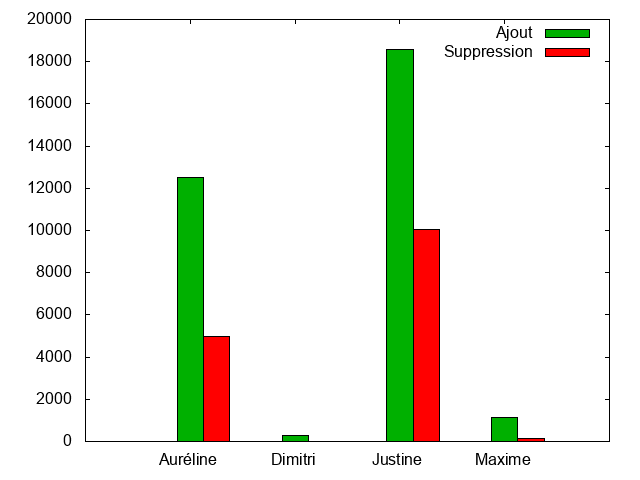
\includegraphics[width=0.66\textwidth, keepaspectratio]{img/repo_stats.png}
			\caption{Nombre de lignes d'ajoutés et supprimés par personnes}
		\end{figure}

	\section{Idées d'améliorations}

		Notre application n'ayant pu être terminé faute de temps, voici la liste des améliorations que nous aurions voulus faire et celles qui seraient possibles d'implémenter ensuite :

		\begin{itemize}
			\item{Concevoir deux types de fichier, l'un pour l'éditeur et l'autre pour le jeu. Le jeu serait une version épurée de celui de l'éditeur et ne contiendrait pas la position des noeuds par exemple}
			\item{Une mise à jour d'un noeud transfert correctement les différents liens (au lieu de les supprimer dans la plupart des cas)}
			\item{Vérifier que le livre est valide pour être joué}
			\item{Créer une classe mère pour les listes sur le côté gauche de l'application (Item et personnage)}
			\item{Une fois la classe mère codé, ajouter une liste à gauche pour gérer les skills dans l'éditeur}
			\item{Déclencher plus d'exception si le livre est incorrect}
			\item{Gérer les shops(jeu et gui), champs auto (jeu uniquement)}
			\item{Afficher les personnages et items inutilisés}
			\item{Indiquer si l'estimation de la difficulté est à jour ou non}
			\item{Gestion des prérequis sur les boites de dialogue des liens}
			\item{Améliorer l'intelligence de la fourmis (pouvoir estimer si un item est plus important qu'un autre, meilleure gestion des combats, ...)}
			\item{Ajouter et supprimer des skills au fil du jeu}
			\item{Ajout de paramètres aux skills (plutot que d'avoir un simple nom)}
			\item{Afficher les chemins gagnants}
			\item{Enlever ou ajouter une somme d'argent à un personnage se fait sur une monnaie précise (ex : -5 dollards, +15 euros, etc)}
			\item{"Langage" simple permettant de manier des conditions et variables pour des prérequis notamment}
			\item{Possibilité d'avoir des pnj qui pourraient nous suivre dans l'aventure pour combattre ou pour dévérouiller certains passages par exemple.}
		\end{itemize}

	\section{Bugs et problèmes connus}

		Certains et problèmes sont connus, en voici une liste non exhaustive une fois de plus :

		\begin{itemize}
			\item{Tests incomplets sur le Book et le Jeu}
			\item{Le changement d'id d'un personnage ou d'un item ne met pas à jour les différents élements du livre (noeuds, choix, ...)}
			\item{Diverses bugs visuels concernant la boite de dialogue sur le Prélude}
			\item{Le zoom ne se fait pas selon la position actuel de la souris mais du point supérieur gauche du GraphPane}
		\end{itemize}
